\documentclass{standalone}
\usepackage{tikz}
\usetikzlibrary{patterns, positioning}
\usepackage[sfdefault]{ClearSans} %% option 'sfdefault' activates Clear Sans as the default text font
\usepackage[T1]{fontenc}

\begin{document}
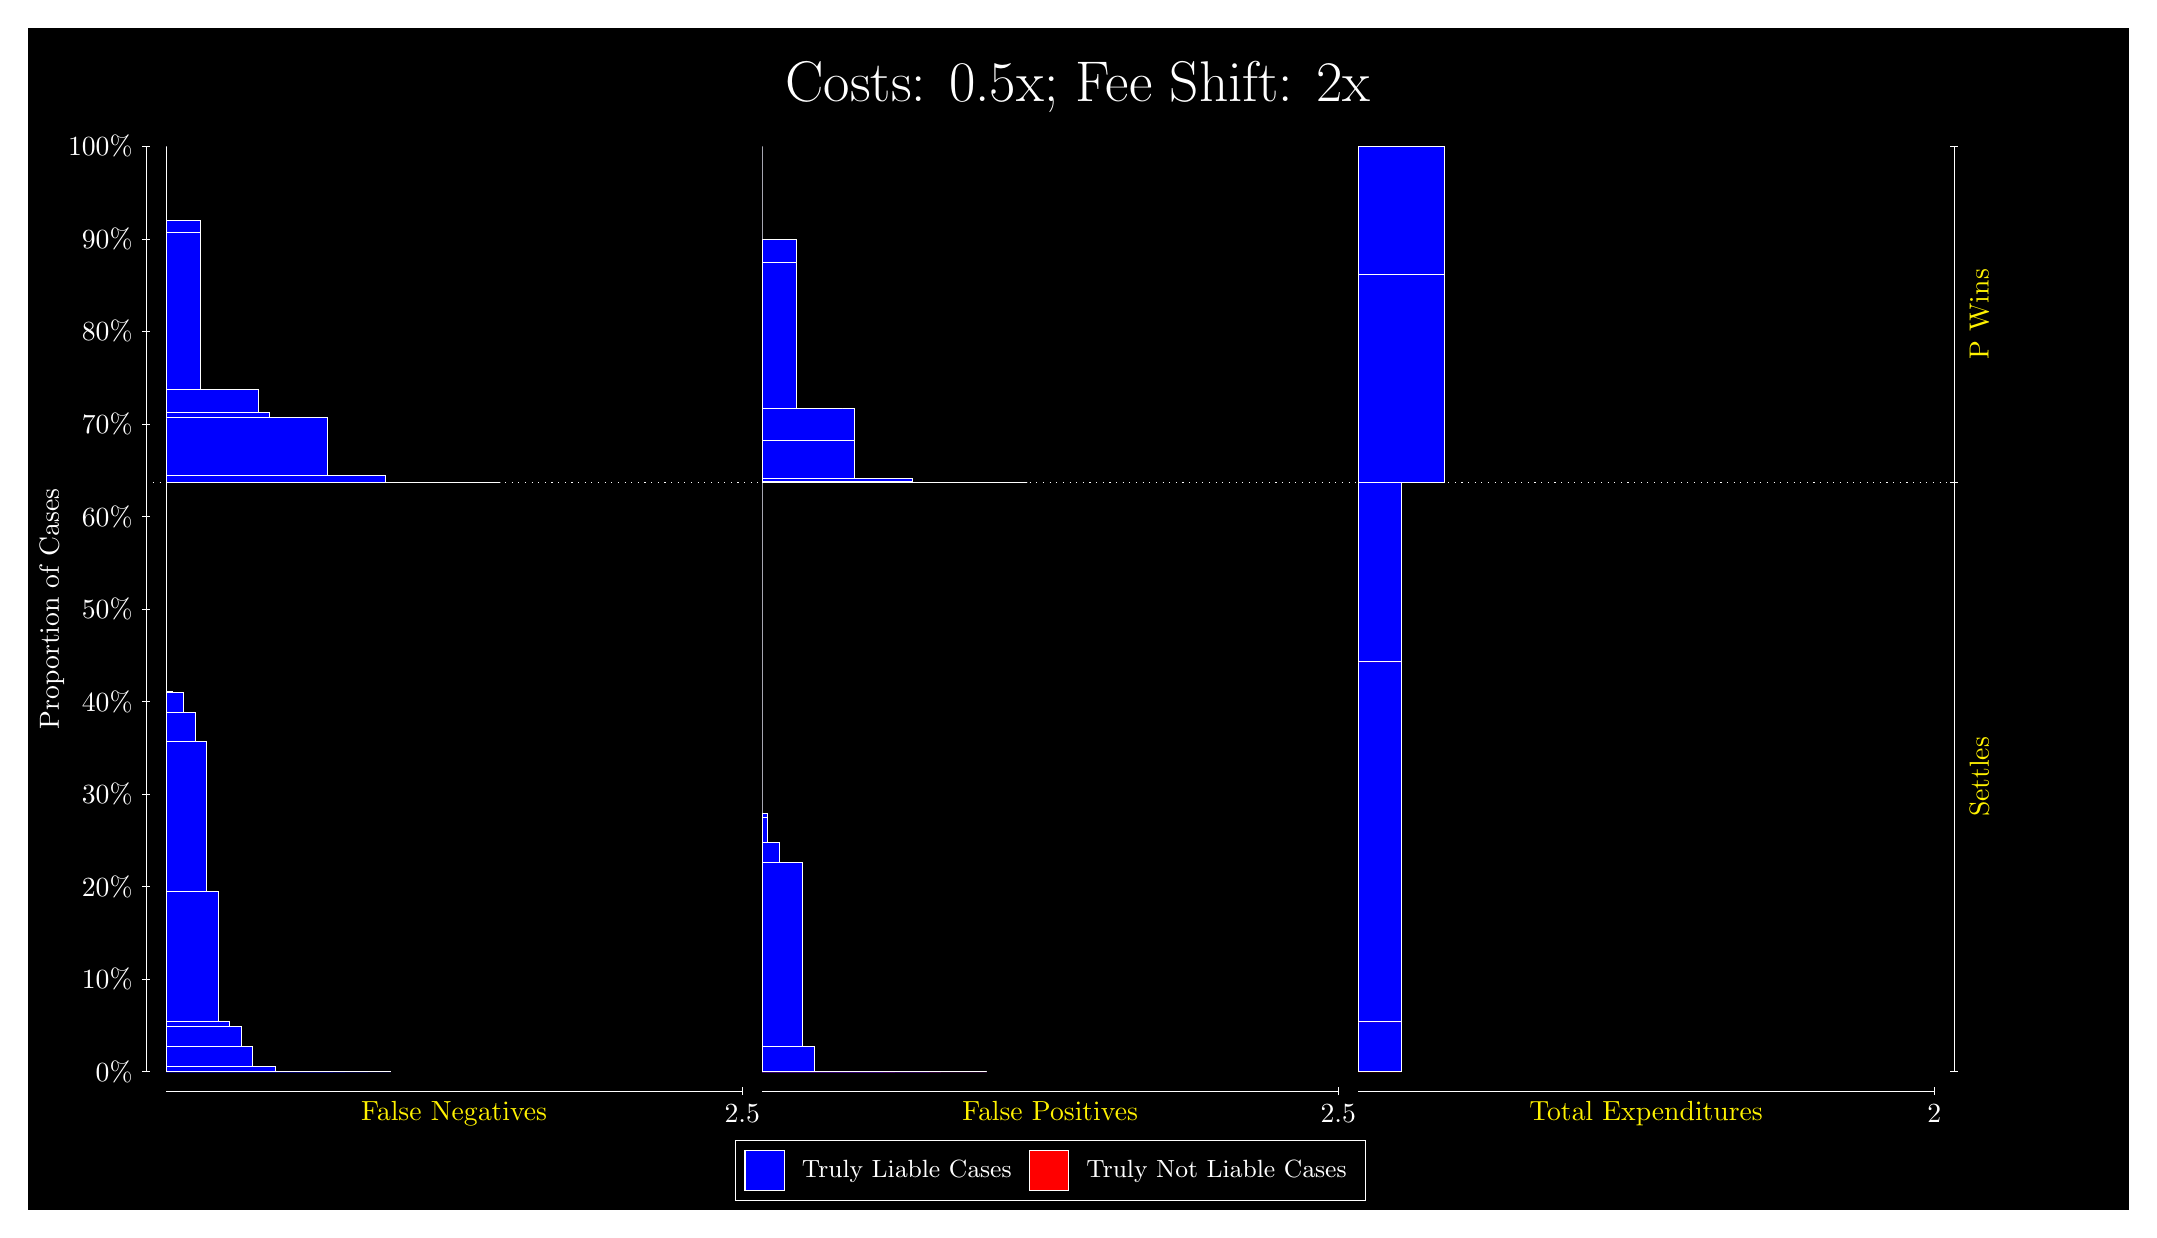
\begin{tikzpicture}
\draw[fill=black] (0,0) rectangle (26.667,15);
\draw[text=white] (0,13.5) rectangle (26.667,15) node[midway] {\huge Costs: 0.5x; Fee Shift: 2x};
\draw[white, very thin] (1.5,1.75) -- (1.5,13.5);
\node[rotate=90, text=white, anchor=center] at (0.3, 7.625) {Proportion of Cases};
\draw[white, very thin] (1.45,1.75) -- (1.55,1.75);
\node[text=white, anchor=east] at (1.45, 1.75) {0\%};
\draw[white, very thin] (1.45,2.925) -- (1.55,2.925);
\node[text=white, anchor=east] at (1.45, 2.925) {10\%};
\draw[white, very thin] (1.45,4.1) -- (1.55,4.1);
\node[text=white, anchor=east] at (1.45, 4.1) {20\%};
\draw[white, very thin] (1.45,5.275) -- (1.55,5.275);
\node[text=white, anchor=east] at (1.45, 5.275) {30\%};
\draw[white, very thin] (1.45,6.45) -- (1.55,6.45);
\node[text=white, anchor=east] at (1.45, 6.45) {40\%};
\draw[white, very thin] (1.45,7.625) -- (1.55,7.625);
\node[text=white, anchor=east] at (1.45, 7.625) {50\%};
\draw[white, very thin] (1.45,8.8) -- (1.55,8.8);
\node[text=white, anchor=east] at (1.45, 8.8) {60\%};
\draw[white, very thin] (1.45,9.975) -- (1.55,9.975);
\node[text=white, anchor=east] at (1.45, 9.975) {70\%};
\draw[white, very thin] (1.45,11.15) -- (1.55,11.15);
\node[text=white, anchor=east] at (1.45, 11.15) {80\%};
\draw[white, very thin] (1.45,12.325) -- (1.55,12.325);
\node[text=white, anchor=east] at (1.45, 12.325) {90\%};
\draw[white, very thin] (1.45,13.5) -- (1.55,13.5);
\node[text=white, anchor=east] at (1.45, 13.5) {100\%};

\draw[white, very thin] (24.457,1.75) -- (24.457,13.5);
\draw[white, very thin] (24.407,1.75) -- (24.507,1.75);
\node[anchor=west] at (24.407, 1.75) {};
\draw[white, very thin] (24.407,9.2347) -- (24.507,9.2347);
\node[anchor=west] at (24.407, 9.2347) {};
\draw[white, very thin] (24.407,13.5) -- (24.507,13.5);
\node[anchor=west] at (24.407, 13.5) {};

\draw[white, very thin, fill=blue] (1.75,1.75) rectangle (4.6044,1.75);
\draw[white, very thin, fill=blue] (1.75,1.75) rectangle (4.3116,1.75);
\draw[white, very thin, fill=blue] (1.75,1.75) rectangle (4.0188,1.75);
\draw[white, very thin, fill=blue] (1.75,1.75) rectangle (3.8725,1.75);
\draw[white, very thin, fill=blue] (1.75,1.75) rectangle (3.5797,1.7505);
\draw[white, very thin, fill=blue] (1.75,1.7505) rectangle (3.4333,1.7512);
\draw[white, very thin, fill=blue] (1.75,1.7512) rectangle (3.287,1.7534);
\draw[white, very thin, fill=blue] (1.75,1.7534) rectangle (3.1406,1.8125);
\draw[white, very thin, fill=blue] (1.75,1.8125) rectangle (2.8478,2.0701);
\draw[white, very thin, fill=blue] (1.75,2.0701) rectangle (2.7015,2.3237);
\draw[white, very thin, fill=blue] (1.75,2.3237) rectangle (2.5551,2.3823);
\draw[white, very thin, fill=blue] (1.75,2.3823) rectangle (2.4087,4.045);
\draw[white, very thin, fill=blue] (1.75,4.045) rectangle (2.2623,5.9487);
\draw[white, very thin, fill=blue] (1.75,5.9487) rectangle (2.1159,6.3184);
\draw[white, very thin, fill=blue] (1.75,6.3184) rectangle (1.9696,6.5713);
\draw[white, very thin, fill=blue] (1.75,6.5713) rectangle (1.8232,6.574);
\draw[white, very thin, fill=red] (1.75,6.574) rectangle (1.75,6.574);
\draw[white, very thin, fill=blue] (1.75,6.574) rectangle (1.75,9.2347);
\draw[white, very thin, fill=blue] (1.75,9.2347) rectangle (5.9949,9.2347);
\draw[white, very thin, fill=blue] (1.75,9.2347) rectangle (5.2631,9.2357);
\draw[white, very thin, fill=blue] (1.75,9.2357) rectangle (4.5312,9.3266);
\draw[white, very thin, fill=blue] (1.75,9.3266) rectangle (4.3848,9.3266);
\draw[white, very thin, fill=blue] (1.75,9.3266) rectangle (3.7993,10.056);
\draw[white, very thin, fill=blue] (1.75,10.056) rectangle (3.6529,10.056);
\draw[white, very thin, fill=blue] (1.75,10.056) rectangle (3.0674,10.117);
\draw[white, very thin, fill=blue] (1.75,10.117) rectangle (2.921,10.413);
\draw[white, very thin, fill=blue] (1.75,10.413) rectangle (2.3355,10.413);
\draw[white, very thin, fill=blue] (1.75,10.413) rectangle (2.1891,12.404);
\draw[white, very thin, fill=blue] (1.75,12.404) rectangle (2.1891,12.563);
\draw[white, very thin, fill=red] (1.75,12.563) rectangle (1.75,12.563);
\draw[white, very thin, fill=blue] (1.75,12.563) rectangle (1.75,13.5);
\draw[white, very thin, fill=red] (9.3189,1.75) rectangle (12.173,1.75);
\draw[white, very thin, fill=blue] (9.3189,1.75) rectangle (12.173,1.75);
\draw[white, very thin, fill=red] (9.3189,1.75) rectangle (11.588,1.75);
\draw[white, very thin, fill=blue] (9.3189,1.75) rectangle (11.588,1.75);
\draw[white, very thin, fill=blue] (9.3189,1.75) rectangle (11.441,1.75);
\draw[white, very thin, fill=red] (9.3189,1.75) rectangle (11.002,1.75);
\draw[white, very thin, fill=blue] (9.3189,1.75) rectangle (11.002,1.75);
\draw[white, very thin, fill=blue] (9.3189,1.75) rectangle (10.856,1.75);
\draw[white, very thin, fill=blue] (9.3189,1.75) rectangle (10.709,1.7505);
\draw[white, very thin, fill=red] (9.3189,1.7505) rectangle (10.417,1.7505);
\draw[white, very thin, fill=blue] (9.3189,1.7505) rectangle (10.417,1.7505);
\draw[white, very thin, fill=blue] (9.3189,1.7505) rectangle (10.27,1.751);
\draw[white, very thin, fill=red] (9.3189,1.751) rectangle (10.124,1.751);
\draw[white, very thin, fill=blue] (9.3189,1.751) rectangle (10.124,1.7548);
\draw[white, very thin, fill=blue] (9.3189,1.7548) rectangle (10.124,1.7569);
\draw[white, very thin, fill=blue] (9.3189,1.7569) rectangle (9.9776,2.0683);
\draw[white, very thin, fill=red] (9.3189,2.0683) rectangle (9.8312,2.0683);
\draw[white, very thin, fill=blue] (9.3189,2.0683) rectangle (9.8312,4.4108);
\draw[white, very thin, fill=blue] (9.3189,4.4108) rectangle (9.6848,4.4134);
\draw[white, very thin, fill=blue] (9.3189,4.4134) rectangle (9.5384,4.6663);
\draw[white, very thin, fill=blue] (9.3189,4.6663) rectangle (9.3921,4.9777);
\draw[white, very thin, fill=blue] (9.3189,4.9777) rectangle (9.3921,5.036);
\draw[white, very thin, fill=blue] (9.3189,5.036) rectangle (9.3189,9.2347);
\draw[white, very thin, fill=red] (9.3189,9.2347) rectangle (12.686,9.2347);
\draw[white, very thin, fill=blue] (9.3189,9.2347) rectangle (12.686,9.2347);
\draw[white, very thin, fill=red] (9.3189,9.2347) rectangle (11.954,9.2347);
\draw[white, very thin, fill=blue] (9.3189,9.2347) rectangle (11.954,9.2347);
\draw[white, very thin, fill=blue] (9.3189,9.2347) rectangle (11.954,9.2349);
\draw[white, very thin, fill=red] (9.3189,9.2349) rectangle (11.222,9.2349);
\draw[white, very thin, fill=blue] (9.3189,9.2349) rectangle (11.222,9.2435);
\draw[white, very thin, fill=blue] (9.3189,9.2435) rectangle (11.222,9.282);
\draw[white, very thin, fill=red] (9.3189,9.282) rectangle (10.49,9.282);
\draw[white, very thin, fill=blue] (9.3189,9.282) rectangle (10.49,9.7668);
\draw[white, very thin, fill=blue] (9.3189,9.7668) rectangle (10.49,10.172);
\draw[white, very thin, fill=red] (9.3189,10.172) rectangle (10.344,10.172);
\draw[white, very thin, fill=blue] (9.3189,10.172) rectangle (10.344,10.172);
\draw[white, very thin, fill=blue] (9.3189,10.172) rectangle (9.758,12.029);
\draw[white, very thin, fill=blue] (9.3189,12.029) rectangle (9.758,12.322);
\draw[white, very thin, fill=red] (9.3189,12.322) rectangle (9.6116,12.322);
\draw[white, very thin, fill=blue] (9.3189,12.322) rectangle (9.6116,12.322);
\draw[white, very thin, fill=blue] (9.3189,12.322) rectangle (9.6116,12.322);
\draw[white, very thin, fill=red] (9.3189,12.322) rectangle (9.3189,12.322);
\draw[white, very thin, fill=blue] (9.3189,12.322) rectangle (9.3189,13.5);
\draw[white, very thin, fill=red] (16.888,1.75) rectangle (17.437,1.75);
\draw[white, very thin, fill=blue] (16.888,1.75) rectangle (17.437,2.3837);
\draw[white, very thin, fill=red] (16.888,2.3837) rectangle (17.437,2.3837);
\draw[white, very thin, fill=blue] (16.888,2.3837) rectangle (17.437,6.9556);
\draw[white, very thin, fill=red] (16.888,6.9556) rectangle (17.437,6.9556);
\draw[white, very thin, fill=blue] (16.888,6.9556) rectangle (17.437,9.2347);
\draw[white, very thin, fill=red] (16.888,9.2347) rectangle (17.986,9.2347);
\draw[white, very thin, fill=blue] (16.888,9.2347) rectangle (17.986,11.881);
\draw[white, very thin, fill=red] (16.888,11.881) rectangle (17.986,11.881);
\draw[white, very thin, fill=blue] (16.888,11.881) rectangle (17.986,13.5);
\draw[white, dotted] (1.5,9.2347) -- (24.457,9.2347);
\draw[white, very thin] (1.75,1.5) -- (9.0689,1.5);
\node[text=yellow, anchor=north] at (5.4094, 1.5) {False Negatives};
\draw[white, very thin] (9.0689,1.45) -- (9.0689,1.55);
\node[text=white, anchor=north] at (9.0689, 1.45) {2.5};

\draw[white, very thin] (9.3189,1.5) -- (16.638,1.5);
\node[text=yellow, anchor=north] at (12.978, 1.5) {False Positives};
\draw[white, very thin] (16.638,1.45) -- (16.638,1.55);
\node[text=white, anchor=north] at (16.638, 1.45) {2.5};

\draw[white, very thin] (16.888,1.5) -- (24.207,1.5);
\node[text=yellow, anchor=north] at (20.547, 1.5) {Total Expenditures};
\draw[white, very thin] (24.207,1.45) -- (24.207,1.55);
\node[text=white, anchor=north] at (24.207, 1.45) {2};

\node[text=yellow, centered, rotate=90] at (24.777, 5.4924) {Settles};
\node[text=yellow, centered, rotate=90] at (24.777, 11.367) {P Wins};

\draw (12.978300999999998,1.5) node[draw=none] (baseCoordinate) {};
\begin{scope}[align=center]
        \matrix[scale=0.5, draw=white, below=0.5cm of baseCoordinate, nodes={draw}, column sep=0.1cm]{
            \node[rectangle, draw, minimum width=0.5cm, minimum height=0.5cm, fill=blue] {}; &
            \node[draw=none, font=\small, text=white] (B) {Truly Liable Cases}; &
            \node[rectangle, draw, minimum width=0.5cm, minimum height=0.5cm, fill=red] {}; &
            \node[draw=none, font=\small, text=white] (B) {Truly Not Liable Cases}; \\
            };
\end{scope}

\end{tikzpicture}
\end{document}